\section{Ziele}
Mithilfe des Versuchs soll die Comptonwellenlänge $\lambda_{\text{C}}$ für ein Elektron bestimmt werden.

\section{Theoretische Grundlagen}
\label{sec:theorie}

\subsection{Compton Effekt}
Wenn Röntgernstrahlung mit Atomen wechseleirkt kommt es zum sogenannten Compton Effekt.
Für den Compton Effekt sind nur die Wechselwirkungen von Photonen mit Elektriónen interessant.
Beim zuammentreffen des Photons mit einem fest gebundenen Elektronen auf einer inneren Schale des Atoms findet eine quasi Reflexion des Photons statt und es gibt keinen merklichen Unterschied in der Wellenlänge.
Wenn das Photon allerdings mit einem freien Elektron in einer äußeren Schale des Atoms regiert findet der Compton Effekt Abb. (\ref{fig:Compton_Effekt}) statt und die "Teilchen" werden gestreut.
Durch die Streuung gibt das Photon Energie an das Elektron ab und seine Wellenlänge vergrößert sich (Gl. \ref{eqn:Photon_Energie}).
\begin{equation}
    E_{\text{Photon}} = \frac{hc}{\lambda} \label{eqn:Photon_Energie}
\end{equation}
Die Differenz der Wellenlänge folgt dabei folgendem Gesetz:
\begin{equation}
    \Delta \lambda = \lambda_2 - \lambda_1
                    = \frac{h}{m_e c}\left( 1- \cos \theta \right) 
                    = \lambda_{\text{C}} \left( 1- \cos \theta \right) \label{eqn:Compton_Gesetz} 
\end{equation}
Wobei die emittierte Wellenlänge bei $\theta = 0°$ minimal ($\Delta\lambda = 0$) ist und für $\theta = 180°$ maximal ($\Delta\lambda = 2\lambda_{\text{C}}$) wird.
\begin{figure}
    \centering
    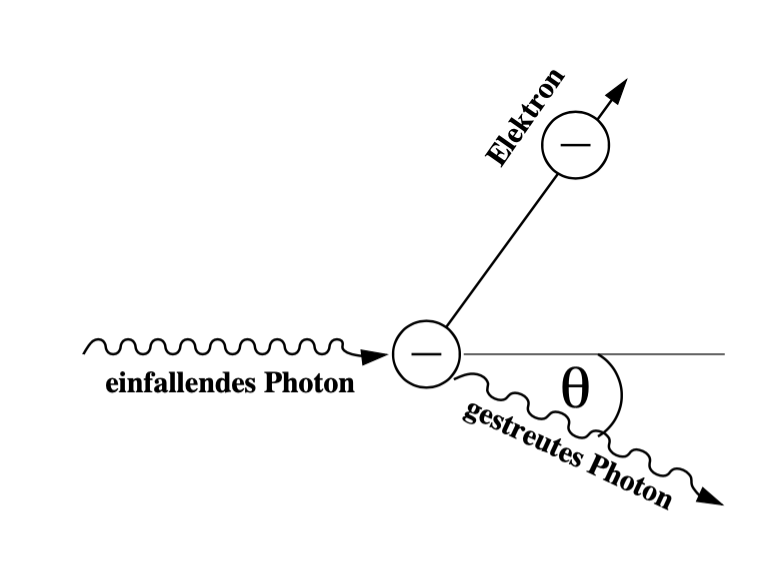
\includegraphics[width=0.7\textwidth]{bilder/Compton_Effekt.png}
    \caption{Wechselwirkung eines Photons mit einem Elektron, das Photon wird im Winkel $\theta$ gestreut}
    \label{fig:Compton_Effekt}
\end{figure}


\subsection{Röntgenquelle}
In einer evakuierten Röhre werden mit einer Glühkathode Elektronen erzeugt und auf eine Kupfer Oberfläche beschleunigt.
Beim auftreffen auf die Kupferoberfläche wird Röntgenstrahlung ausgesandt. Die Röntgenstrahlung setzt sich aus der Bremsstrahlung und charaktersitischen Peaks zusammen.

\subsubsection{Bremsstrahlung}
Beim eintritt in das Kathodenmaterial treten die Elektronen auch in das Coulombfeld der Atomkerne des Kupfers ein.
Im Coulombfeld der Kerne werden die Elektronen abgelenkt und abgebremst, dadurch verringert sich ihre kinetische Energie.
Die Energiedifferenz durch die abbremsung wird in Form von Röntgenstrahlung in einem kontinuierlichen Spektrum abgestrahlt.

\subsubsection{Charakteristische Peaks}
Wenn die Elektronen in das Kathodenmaterial eidringen kann es auch vorkommen dass die Elektronen in den Kupferatomen angeregt werden.
Wenn ein Kupfer-Elektron auf ein höheres Energieniveau angereagt wird gibt es direkt wieder Energie ab um auf den energetisch Günstigeren Zustand zurück zu "fallen".
Beim Rücktritt in den Zustand gibt das Elektron die gerade noch gewonnene Energie in Form eines Röntgenquants wieder ab.
Die Energie der Röntgenstrahlung ist somit durch die Energiedifferenz der Zustände klar definierrt und es enstehen charakteristische Peaks zu den entsprechenden Energien.

\subsection{Transmission}
In Aluminium wird die entstandene Röntgenstrahlung transmittiert als auch Absorbiert, wobei die Transmission Wellenlängenabhängig ist und die Absorption einem exponentiellen Absorptionsgesetz folgt(\ref{eqn:Absorption}).
\begin{equation}
    I = I_0 \cdot e^{-\mu d} \label{eqn:Absorption}
\end{equation}
Wobei $d$ die Materialdicke und $\mu = \mu_{\text{Paar}}+\mu_{\text{Photo}}+\mu_{\text{Compton}}$ der Absorptionskoeffizient ist.
Für die Transmission gilt, dass bei wachsender Wellenlänge die Transmission proportional sinkt.

\subsection{Bragg Reflexion}
Wenn Röntgenstrahlung auf ein dreidimensionales regelmäßiges Kristallgitter fällt findet die sogenannte Bragg-Reflexion statt.
Wenn die Röntgenstrahlung auf den Kristall fällt wird sie in verschieden tiefen Netzebenen des Kristalls refelektiert und wenn ein Gangunterschied der ungleich einem vielfachen der Wellenlänge der einfallenden Strahlung ist auftritt dann entsteht durch die große Anzahl der Ebenen destruktive interferenz und die Strahlungsintensität nimmt strk ab.
Falls der Entrittswinkel allerdings genau dem Bragg-Winkel (nach Gl. \ref{eqn:Bragg_Gleichung}) entspricht findet zwischen den Ebenen konstruktive Interferenz statt und die Strhlung wird mit gleicher Intensität emittiert.
\begin{equation}
    n\lambda = 2 d \sin(\alpha) \label{eqn:Bragg_Gleichung}
\end{equation}
Bragg Gleichung mit der Beugungsordnung $n$ ,dem Gitterabstand $d$ (siehe Abb. \ref{fig:Bragg_Reflexion}) und dem Glanzwinkel $\alpha$ (siehe Abb. \ref{fig:Bragg_Reflexion}).
\begin{figure}
    \centering
    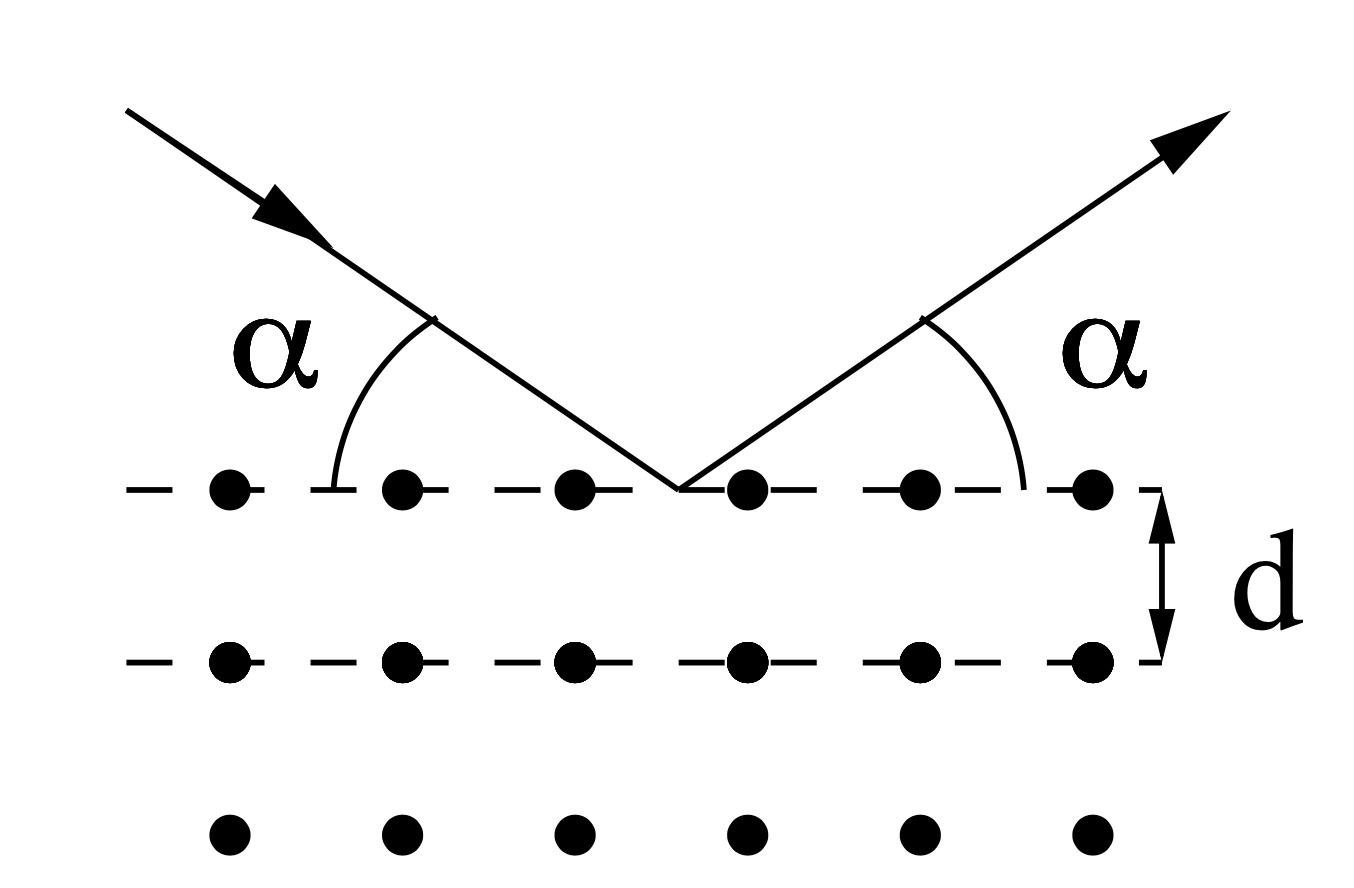
\includegraphics[width=0.7\textwidth]{bilder/Bragg_Reflexion.png}
    \caption{Bragg Reflexion im Winkel $\alpha$ an einem Kristallgitter mit Gitterabstand $d$ }
    \label{fig:Bragg_Reflexion}
\end{figure}
\subsection{Geiger Müller Zählrohr}


